\chapter{相关技术}
% \label{chap:intro}

\section{基于相关规则的推理}

公式化的规则作为一种比较常见的方法,常常被应用于对知识的表示以及推理准则的描述之中\cite{Ligeza2006Logical}。公式化的规则最明显的特点就是便于理解,它通常把一个又一个的规则抽象成为一个公式,这个公式可以用以下蕴含式表示:

\begin{equation}
if<condition...>then<conclusion>
\end{equation}

这个蕴含表达式中的前件式<condition...>表示的是一个规则中的条件部分。他可以是某一个条件,也可以是多个条件构成的并集。对于多种条件的规则,可以使用析取、合取或者否定等逻辑规则将这些条件组合成为一个逻辑公式。这个蕴含表达式的后件式是<conclusion>,他表示前件式中的规则所对应的结果。所谓的规则触发指得是一旦前件被满足,便会得到后件式中对应的推理结果。通常情况下,规则可以由某专业领域的知识构成。

在人工智能领域,专家系统是一种具有模拟人类专家决策能力的计算机系统,它是基于规则的推理(Rule Based Reasoning)的一种典型的应用\cite{Buchanan1984Rule,Gonzalez1985The}。专家系统旨在通过知识系统(主要表现为规则)来推理,而不是通过常规的程序代码来解决复杂的问题。世界上第一个专家系统叫做DENDRAL创建于19世纪70年代\cite{Grabiner1986Computers}, 该专家系统被应用化学领域。在1980年代,业界对专家系统的相关研究激增。 大学提供了专家系统课程,世界五百强公司中有三分之二将这项技术应用于日常商业活动。日本的第五代基于专家系统的计算机操作系统项目曾一度引起了国际关注\cite{Mccampbell1999Knowledge,Durkin:1996:ESV:629551.630145}。第一个应用于智能医疗领域的专家系统是MYCIN\cite{Shortliffe1976Copyright}, EMYCIN在MYCIN的基础上增加了命令行工具\cite{Buchanan1984Rule}。

专家系统作为一个基于规则的推理方法的商业系统,主要由两大部分构成:知识库以及规则引擎\cite{Friedland1985Special}。

\begin{itemize}
\item \textbf{}知识库代表有关世界的事实。在诸如Mycin和Dendral的早期专家系统中,这些事实主要表示为关于变量的断言。在后来使用商业外壳开发的专家系统中,知识库采用了更多的结构,并使用了面向对象编程中的概念。世界被表示为类,子类,实例和断言被对象实例的值代替。规则通过查询和声明对象的值来工作。
\item \textbf{}推理引擎是一个自动推理系统,可以评估知识库的当前状态,应用相关规则,然后将新知识断言到知识库中。推理引擎还可以包括解释能力,以便可以通过追溯导致断言的规则的发散,向用户解释用于得出特定结论的推理链。\cite{Hayes1983Building}

\end{itemize}

推理引擎有两大主流模式:前向链接和后向链接。两种模型的主要区别在于推理引擎是由规则的前驱还是后继驱动。 在前向链接中,前一个条件会触发后件中的声明结果。 例如,考虑以下规则:

\begin{equation}
R1:Man(x) \Rightarrow Mortal(x)
\end{equation}

前向链接的一个简单示例是将Man(x)声明给系统,然后触发推理引擎。 它将匹配规则R1并将Mortal(x)最为推理结果。而后向链接不太直接。 在后向链接中,推理引擎查看可能的结论并检查推理是否正确。 因此,如果系统试图确定Mortal(x)是否为真,它将找到R1并查询规则以查看Man(x)是否为真。 专家系统的早期创新之一是将推理引擎与用户界面集成在一起。 对于反向链接,此功能尤其强大。系统可以在街面上展示预期的目标,并指引用户进行规则以及数据的匹配。

公式化的规则的来源主要有两个途径。一个是对专业领域内的相关文献或者领域内的专家的相关经验进行翻译。另一个则是使用人工智能的相关算法\cite{Mitchell1997Machine}在大量的数据集中进行学习而归纳出来的,比较经典的构造算法例如ID3算法\cite{Quinlan1986Induction}。

\subsection{基于相关规则的推理的优点}

\begin{itemize}

\item \textbf{简洁性}

基于相关规则的推理将从专业领域相关文献或者专家的知识抽象化成为公式化的规则,并把规则也结论整理成为一个简单的蕴含关系。规则中的各个条件相对独立没有干扰,当某个条件发生变化需要修改规则时,其他条件一般不需要被修改。

\item \textbf{模块化}

不同于基于相关规则的推理的简洁性,不同的规则之间的关系也是相对独立的。当一个规则整体发生变化时,该规则可以直接在知识库中发生修改而不依赖于其他规则。这种规则本身模块化的属性使得给予规则推理的系统具有较高的可维护性。

\item \textbf{系统易于维护}

基于知识的系统的目标是使系统正常运行所需的关键信息变得清晰。在传统的计算机程序中\cite{Biles1983Building},逻辑嵌入在代码中,通常只能由工程师进行检查。对于基于规则推理的系统,目标是以一种直观,易于理解,查看甚至由领域专家而非工程师编辑的格式指定规则。这种明确的知识表示的好处是有利于系统的不断迭代和易于维护。

\item \textbf{可解释性强}

基于相关规则的推理,整个过程都具有可解释性并对使用者透明。领域专家可根据公式化规则得知每个决策做出的原因。这对于某些领域是非常重要的,比如医疗领域,医生必须知道决策结果是根据哪条医疗规范,以确保治疗的精确性与安全性。

\end{itemize}

\subsection{基于相关规则的推理的缺点}



\begin{itemize}

\item \textbf{规则难以获取}

获取公式化的规则的一个主要方法是对专业领域内的相关文献或者领域内的专家的相关经验进行翻译。一般领域的专家资源比较宝贵,如果想从领域专家的知识中获得规则,可能导致较高的成本。同时,考虑到将专家知识转化为可以利用的规则,翻译人员的水平可能导致信息的损失。这可能导致规则本身的偏差,直接影响到推理的效果。这使得对基于规则的推理系统的大量研究经历都放在如何实现知识获取工具上。获取公式化的规则的一个主要方法是使用人工智能的在大量的数据集中进行学习,这种方法的问题在于如此大量的经过标注的数据集难以获得;同时,考虑到数据集可能不均匀的特点,许多不常用的规则难以被算法学习到。另外有一些领域,例如医疗等,这些领域专业性强且十分复杂,每个决策的给出需要依赖大量的文献以及理论研究支撑,这可能导致这些领域需要大量的公式化规则,进一步加大知识的获取难度。

\item \textbf{规则的匹配速度问题}

对某条规则的匹配速度无疑制约着系统的性能。在早期,对专家系统的研究主要集中在环境部署上。但当系统的知识库不断增加,推理的规模问题成为了系统最主要的挑战。尽管有许多规则匹配算法来优化匹配速度,比如Rete算法\cite{Hunt2005Effects},该算法通过改善专家系统中的推理引擎来优化推理速度,但其本质依然是将带推理的样本于整个知识库中的所有规则进行匹配。随着知识库的不断扩展,计算的规模依然会变得很大。因此这类算法针对规则库的扩充往往束手无策。

\item \textbf{知识库难以迭代或者更新}

通常情况下随着一个领域内研究的不断深入,该领域的知识库可能发生改变。这类似于机器学习中概念漂移的概念\cite{article}。领域中知识的变化,新知识的出现,可能导致知识库中某些规则的条件需要增加或者删除,甚至可能导致某一些规则直接失效。但是知识库却无法拥有自我更新与迭代的能力,于是产生了相应的概念漂移。除非请该领域的专家,不断根据领域内新的经验来维护知识库,该问题无法得到本质上的解决。

\end{itemize}



\section{基于数据的推理}
基于数据的推理又称基于案例的推理(case based reasoning, 简称CBR)。对此的研究最早发生在十九世纪八十年代,由耶鲁大学的Roger Schank及其学生首先提出\cite{Schank1982Dynamic}。以此研究为基础衍生出的基于案例的推理的两个系统分别是Janet Kolodner设计的CYRUS\cite{Schank1988SCRIPTS,LebowitzGeneralization}以及 Michael Lebowitz设计的IPP\cite{Lebowitz2005Memory}。

广义上来说,基于案例的推理是一个基于相似历史问题的解决方案来解决新问题的过程。其基本的原理是将海量的历史案例以及相应的解决方案构成一个知识库,当对一个新的样本做分析推荐时,依照一些算法,在知识库中搜寻出最为相似的几个历史案例,并根据这些案例进行进一步的决策。再完成推理后,系统还要根据专家意见决定是否修改新样本的解决方案,并决定是否将该样本纳入数据库。

基于案例的推理按照目的不同可以分为四个阶段,这四个阶段构成一个CBR循环\cite{Aamodt2001Case}。这里,本文结合一个例子分别介绍这四个阶段:

\begin{enumerate}
  \item \textbf{检索阶段}
  
  在检索阶段给定目标问题,请从内存中检索与解决问题有关的案例。一个案例包括一个问题,其解决方案,以及通常包含有关解决方案来源的注释。例如,假设弗雷德想要准备蓝莓煎饼。作为一个新手厨师,他能回忆到的最相关的经验是他成功地制作了薄煎饼。他遵循的制作薄煎饼的程序,以及沿途做出决定的理由,构成了弗雷德的案例。
  \item \textbf{重用阶段}
  
  将解决方案从先前的案例映射到目标问题。这可能涉及根据需要适应解决方案以适应新情况。在薄煎饼示例中,Fred必须修改他检索到的解决方案,以包括添加蓝莓。
  \item \textbf{修订阶段}
  
  将先前的解决方案映射到目标情况后,在现实世界中测试新解决方案(或模拟),并在必要时进行修订。假设弗雷德通过向面糊中添加蓝莓来适应他的煎饼解决方案。混合后,他发现面糊已变成蓝色–这是不希望的效果。这建议进行以下修改:将蓝莓的添加延迟到面糊倒入锅中之后。
  \item \textbf{保留阶段}
  
  解决方案已成功适应目标问题后,将得到的经验作为新案例存储在内存中。因此,弗雷德记录了他制作蓝莓煎饼的新程序,从而丰富了他的存储经验,并为未来的煎饼制作需求作了更好的准备。
\end{enumerate}



\subsection{基于案例推理的主要类型}

CBR循环涵盖了组织,检索,利用过去案例中保留的知识的各种不同方法。案例可以作为具体经验保留,或者一组类似的案例可以构成一个广义的案例集合。案例可以存储为单独的知识单元,也可以拆分为多个子单元并分布在知识结构内。案例也可以通过前缀或开放式词汇来索引,也可以在统一或分层索引结构内进行索引。先前案例的解决方案可以直接应用于当前问题,也可以根据两种案例之间的差异进行修改。案例的匹配,解决方案的调整以及从经验中学习可以基于通用知识的更深层次的模型,或者基于更浅薄的和经过汇编的知识,或者仅基于明显的句法相似性。

CBR方法可能是完全独立的,自动的,或者可能与用户进行大量交互以支持和指导用户做出选择。某些CBR方法在其案例库中假设了大量分布广泛的案例,而其他方法则基于一组较为有限的典型案例。可以顺序地或并行地检索和评估。

实际上,“基于案例的推理”仅仅是用于指代此类系统中一组术语中的一个。“基于案例的推理”是一个集合的概念,而其本身也是一种系统的类型,这容易引起混淆。基于案例的推理有以下几种类型:

\begin{enumerate}
  \item \textbf{基于实例的推理}
  
  这是将基于示例的推理专业化为高度句法的CBR方法。为弥补一般背景知识缺乏的问题,需要相对大量的实例以接近概念定义。实例的表示通常很简单(例如使用特征向量表示),因为基于实例的推理主要的重点是研究CBR循环中不依赖于用户的自动学习。
  \item \textbf{基于内存的推理}
  
  这种方法强调将大量案例收集到内存中,并将推理转化为在此内存中访问和搜索的过程。内存的组织和访问是该方法研究的重点。并行处理技术的利用是基于内存的推理的特征,并将这种方法与其他方法区分开来。
  \item \textbf{基于案例的推理}
  
  尽管本章使用基于案例的推理作为通用术语,但典型的基于案例的推理方法具有一些特性,使其与此处列出的其他方法有所区别。首先,通常假定典型案例中包含一定程度的信息丰富度,并且相对于其内部组织而言具有一定的复杂性,即具有某些值和对应类的特征向量不是所谓的典型案例。典型的基于案例的方法还具有另一个特征:在不同的问题解决环境中应用时,它们能够修改或调整检索到的解决方案。基于范例的基于案例的方法还利用了一般的背景知识,尽管其丰富性,显式表示的程度以及CBR过程中的角色是变化的。典型的CBR系统的核心方法大量借鉴了认知心理学理论。
  
  \item \textbf{基于类推论的推理}
  
  该术语有时被用作基于案例的推理的同义词,用于描述刚刚描述的基于案例的典型方法。然而,它也常被用来表征基于不同领域过去案例解决新问题的方法,而典型案例方法则专注于单领域案例的索引和匹配策略。
\end{enumerate}

\subsection{基于案例的推理的优点}
基于案例的推理有下面几个明显的优点:

\begin{enumerate}
  \item \textbf{处理复杂知识的能力}
  
  基于规则的推理依赖于已经翻译好的规则,但是这些规则往往以来专业人员的翻译与整理,当遇到某些领域内的较为复杂的规则时,这种翻译与整理的准确性难以获得保障;而基于案例的推理通过大量的历史数据来间接的对规则加以解释,保证了准确性。
  \item \textbf{表达方式统一}
  
  对于每一个新的案例的推理都依赖于数据格式相类似的历史案例,这使得对知识的表达更加自然清楚,便于用户浏览与理解。
  \item \textbf{案例单元化}
  
  知识库中的每个历史案例都是相互独立的。因此可以把一个历史案例视为一个基本的存储以及计算单元,在知识库中增加,修改,或者是删除一个基本单元并不会对其他单元造成影响。
  
  \item \textbf{案例易获取}
  
  尽管在一些比较复杂的领域,知识相对匮乏,案例获取相对来说并不容易,比如医疗领域。但对于大多数领域,新案例的获取难度和成本均比较低。
  
  \item \textbf{自我更新能力突出}
  
  当系统对于一个新的等待推理的案例进行分析时,在经历了检索,重用,修正阶段之后,系统可以决定是否将该新案例纳入到知识库中,这样做使得系统的知识库进入了动态变化的状态,使得系统具有自我更新的能力,一定程度上防止了概念漂移的产生。
  
  \item \textbf{鲁棒性强}
  
  以基于数据推理方法为核心的推荐系统具有较高的鲁棒性,这样的系统对信息缺失或输入异常的案例并不敏感。这是因为,一旦一个异常的案例被系统留用,系统仍然可以根据其他与待推理案例相似的历史案例最初正确的推理。
  

\end{enumerate}

\subsection{基于案例的推理的缺点}
基于案例的推理也有下面几个缺点:

\begin{enumerate}
  \item \textbf{对知识的表示缺少普适性}
  
  基于规则的推理源于领域的普适性原则,使用规则对知识进行表达更加通用。而基于案例的推理依赖于历史案例,对知识的表示基本不具有普适性。
  
  \item \textbf{知识往往难以获得}
  
  当案例库中案例的数量和规模大到一定程度,并且不同类别的案例足够均匀时,使用基于案例的推理来获取知识相对容易。但在某些情况下,针对某些较为复杂的领域,知识库的构建本身就是一种挑战。这样的知识库往往案例数量十分有限,或者案例的分布够均匀。此时采用基于案例的推理也许会产生一些问题\cite{Sabater1998Using,Oh2013Introduction}。

\end{enumerate}


\section{决策树算法}

基于相关规则的推理的一个最常见的应用便是决策树算法。决策树算法常常被用来处理分类问题。决策树是一种类似于流程图的结构,其中每个内部节点代表一个属性上的“测试”(例如,硬币翻转是正面还是反面出现),每个分支代表测试的结果,每个叶节点代表一个测试结果。决策树算法同时还是一个算法显示的方法。决策树经常应用于决策分析以及运筹学中,它帮助确定一个能最可能达到目标的策略。一般来说,从根节点到叶子节点的一条路径代表一个分类规则。决策树的输出具有唯一性,如果希望使用决策树算法输出多个决策结果,可以考虑根据决策类型建立多个决策树。

决策树中包含有三种类型的结点:

\begin{enumerate}
  \item \textbf{决策结点},对应于规则中的条件
  \item \textbf{机会结点},表示一棵子树的跟结点,与决策结点相连
  \item \textbf{终结点},用于输出决策结果
\end{enumerate}

决策树是一种用于表达分类规则的递归结构。这样的树的每一个叶子结点可以与一个类别相关联。 该树还可以由具有一组互斥可能结果的机会结点以及每个此类结果的辅助决策树组成。 为了对一个对象进行分类,我们从树的根开始遍历。如果遍历到了叶子结点,则为对象分配与该叶子关联的类。 或者,如果遍历到了机会结点,则根据决策结点确定给定对象的测试结果,然后继续使用与该结果关联的辅助决策树进行处理。因此,通过追踪从决策树的根到其叶子之一的路径来对对象进行分类。

决策树算法的训练集时已知分类的对象集合。归纳学习旨在从大量的经验数据中归纳抽取出一般的判定规则和模式,是从特殊情况推导出一般规则的学习方法。归纳学习的目标是形成合理的能解释已知事实和预见新事实的一般性结论。分类任务是找到一个通用分类规则的问题,该规则在给定训练集中的对象上有很好的效果。根据以上假设,决策树算法在尝试对未知分类的物体进行分类时将很有用。

相对于其他数据挖掘算法,决策树在以下几个方面拥有优势:

\begin{enumerate}
  \item \textbf{决策树易于理解和实现},人们在通过解释后都有能力去理解决策树所表达的意义。
  \item \textbf{对于决策树,数据的准备往往是简单或者是不必要的},其他的技术往往要求先把数据一般化,比如去掉多余的或者空白的属性。
  \item \textbf{能够同时处理数据型和常规型属性},其他的技术往往要求数据属性的单一。
  \item \textbf{是一个白盒模型}如果给定一个观察的模型,那么根据所产生的决策树很容易推出相应的逻辑表达式。
  \item \textbf{易于通过静态测试来对模型进行评测}。表示有可能测量该模型的可信度。
  \item \textbf{在相对短的时间内能够对大型数据源做出可行且效果良好的结果。}
\end{enumerate}

决策树算法的缺点:
\begin{enumerate}
  \item \textbf{模型难以维护},当数据集中有新的样本出现时,需要对模型重新学习,增加了时间成本。考虑领域内的知识发生更新的情况,一般无法在现有的决策树结构中增加新结点或者简单地修改规则,因此往往需要重构整个决策树。
  \item 对于那些各类别样本数量不一致的数据,在决策树当中信息增益的结果偏向于那些具有更多数值的特征。这使得决策树算法对于某些边缘类别的识别束手无策。
\end{enumerate}



为了更直观地介绍决策树算法,考虑下面一个例子:给定一系列普通的对象,每个对象属于且仅属于一个类别,任意两个类别集合交集为空,彼此正交。对象的属性仅通过其属性集合的值确定,因此只有当两个对象在某个属性上的值不相同时,这两个对象才能被区分开。对象的属性可以是离散的,属性值可能是选自某个可能值集合之中;也可以是连续的数字。例如,某一天的天气情况可以用以下几个属性描述:

\begin{itemize}

\item 天气类型。比如某天的天气类型可能是晴天,阴天或者雨天
\item 气温。气温是一个连续的属性
\item 湿度。湿度也是一个连续的属性
\item 是否有风。该属性是离散的,其值之可能是有或者没有

\end{itemize}

某一天的天气情况可以由上述四个属性唯一描述,比如,可以将某一天的天气情况描述为:

\begin{center}
天气类型=多云,气温=38$^{\circ}$C \\
湿度=80\%,是否有风=否 \\
\end{center}

考虑使用某决策树决定这一天是否外出踏青,该决策树的结构如图\ref{fig:ch2-1}所示。根据这棵决策树,这一天的决策结果是:外出。

\begin{figure}[!htp]
  \centering
  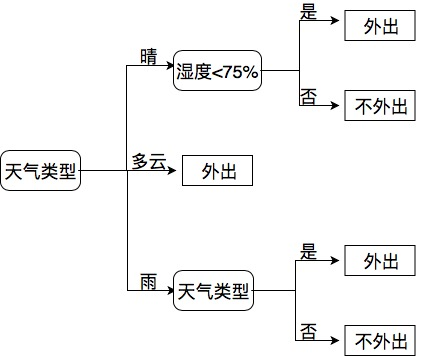
\includegraphics[width=10cm,height=8cm]{figure/决策树.jpg}
  \bicaption[一个典型的决策树]
    {一个典型的决策树}
    {a typical decision tree}
  \label{fig:ch2-1}
\end{figure}


如这棵树所示,通常将每个机会结点限制为单个属性的函数。尽管可以将属性的任何函数用于形成机会结点,但这会带来两个个不良后果:第一,通过在每个阶段检查所有可能的机会结点来构建决策树,无疑要探索路径的计算成本非常大。第二,其中每个机会结点都对应一个功能复杂的决策树可能会使得整个决策树的结构更加复杂。因此,基于树的方法对属性的选择式特别敏感。这里的隐含假设是,定义属性的人为我们提供了用于构建决策树的相关证据支撑。比如在这个例子中,天气,湿度,是否有风等因素都决定着一个人是否应该外出。


\section{kNN算法}


K最近邻(K-nearest neighbors,KNN)算法是一种监督式的机器学习算法,可用于分类以及回归问题。 但是,在工业界它主要用于分类预测问题。 以下两个属性可以很好地描述KNN:

\begin{itemize}

\item \textbf{kNN算法是一种惰性学习算法}

kNN算法对整个训练数据集并没有训练得到一个整体的模型,这样,对于每一个新的测试数据点,都需要根据该点和训练数据集来对目标函数进行预测。kNN算法是“被动的”等待新的测试数据到来,才开始对其进行预测,而不是早早的根据训练数据集把模型建好,对于新的测试数据,只需要往模型中代入就可以得到结果。

\item \textbf{kNN算法是一种非参数学习算法}

对于一个新的数据实例,KNN基于K个最相似的训练模式(已标记的实例),同时保留一些对不可见数据的泛化能力。

\end{itemize}

kNN分类起主要依照特征相似性来对新的样本点进行预测并决定其分类。也就是说,对于一个新的样本点,其预测分类取决于数据集中与其最为相似的K个历史样本。可以将kNN算法大概分为以下几个步骤:

\begin{itemize}

\item \textbf{步骤1} 定义训练集与测试集
\item \textbf{步骤2} 确定K的值,也就是寻找的最邻近的邻居的个数。K可以是任意整数,但K的值一般小于26。
\item \textbf{步骤3} 对测试集中的每一个样本依次执行以下任务:
    \begin{itemize}
    
    \item \textbf{步骤3.1} 计算测试数据与各个训练数据之间的距离。这里的距离实际上度量的是样本之间的相似程度。近来已经提出了许多方法来解决相似度度量的问题,例如欧氏距离,马氏距离和明可夫斯基距离及其变体。对该问题的普遍结论是,不同的应用需要不同的距离测量方法\cite{Quinlan1986Induction,Zhang2006Clustering,ZhuMissing}。
    \item \textbf{步骤3.2} 按照距离由小到大的顺序对所有样本排序。
    \item \textbf{步骤3.3} 找出前k个距离最小,也就是最相似的k个近邻。
    \item \textbf{步骤3.4} 根据这k个近邻进行决策。
    \end{itemize}
\end{itemize}

针对上述步骤3.4,对与kNN算法,当找出待预测的样本在历史样本中最相似的k个样本后,如何进行决策一度成为有关kNN算法研究的热点。其中一个最简单的方法就是采用投票原则:对于分类问题当最邻近的k个邻居确定以后,使用其中数量最多的类别作为决策结果来预测待分类的样本。基于投票原则的决策方法可以用公式\ref{eq2-2}进行表示:

\begin{equation}
\label{eq2-2}
\hat{y}=arg\max_{y_c\in Y} \sum_{{<\Vec{x}^{(i)},y^{(i)}>}\in S(\Vec{x},k)} c(y^{(i)})
\end{equation}

在公式\ref{eq2-2}中,${<\Vec{x}^{(i)},y^{(i)}>}$表示一个训练集;其中的${\Vec{x}^{(i)}}$表示第i个样本点的特征向量,而${y^{(i)}}$表示第i个样本所属的分类。Y表示所有可能的分类所构成的集合。${\Vec{x}}$表示待预测的样本点的特征向量;${\hat(y)}$表示待遇的的样本点的目标类别。
${S(\Vec{x},k)}$表示案例库中与样本${\Vec{x}}$最为相似的k个样本点构成的集合。函数c是一个指示函数,其含义如公式\ref{eq2-3}所示。

\begin{equation}
\label{eq2-3}
c(y^{(i)})=
\begin{cases}
1& {y^{(i)}=y_c}\\
0& {y^{(i)} \ne y_c}
\end{cases}
\end{equation}

考虑将kNN算法应用于回归问题的情形,此时对未知样本的输出并不在是一个离散类型的分类,而应该是一个连续函数,因此考虑将公式\ref{eq2-2}改写为公式\ref{eq2-4}的形式。其中的分式$\frac{1}{k}$表示了投票原则,待预测样本的k个最相似近邻对最终的目标函数具有相同的贡献。



\begin{equation}
\label{eq2-4}
\hat{y}=\frac{1}{k} \sum_{{<\Vec{x}^{(i)},y^{(i)}>}\in S(\Vec{x},k)} y^{(i)}
\end{equation}

上述针对knn算法步骤3.4所采用的基于简单投票准则的决策方法是一种非常简单,易于理解与实现的方法,其核心的思想概括为“少数服从多数”,这种想法是基于与待预测样本的最相似的k个样本具有相同的权重,显然这种思想在一定成度上缺乏合理性。直观上看,距离越近的样本,具有更高的相似度,它在最后的决策中应该发挥更重要的作用;距离越远的样本,具有较低的相似度,它在最后的决策中应该发挥较轻的作用。有许多研究仔细探讨过对步骤3.4的优化,比如文献\parencite[]{ShenFuzzy,Rosa2003Data,RenThe}使用了模糊数学的理论来优化决策过程,而文献\parencite{Ali2011Improved}考虑采用Dempster Shafer证据理论进行决策。本文在第四章考虑引入标签不确定度来优化决策过程。

相比于其他方法,kNN算法有以下几个优点:
\begin{itemize}

\item knn算法最大的优点就是可解释性强,算法输出预测结果后使用者可以直观的知道算法是依据哪些临近样本做出的这样的决策。这在某些领域显得特别重要,比如医疗。使用knn算法为病人推荐治疗方案。医生可以追本溯源,查案历史类似病例,辅助医生做出更好的判断。

\item kNN是一种惰性学习算法,它不需要从一开始进行训练,而仅仅是在待预测样本到来时才进行预测,这减少了训练模型的开销。

\item kNN算法是非参数的学习算法这一特点使得它对于训练集的分布是否均匀并不敏感。

\end{itemize}

knn也存在着几个不容忽视的缺点:

\begin{itemize}

\item kNN算法最大的问题就是计算开销比较大。对于每一个待预测的样本,kNN算法都要将其与所有训练集中的样本进行比较确定相似度。随着知识库的不断积累,计算的规模也在不断的增加,时间与空间成本都会显著提升。近来有许多研究提出使用近似算法来优化kNN算法,以达到计算准确度与时间空间复杂度之间的折中。比如文献\parencite{MathyThe}使用了边界树算法来优化kNN算法,在本文的第4章还将详细讨论。

\item k值的选取也对kNN算法的影响比较大,因此也一度成为有关kNN算法的研究热点\cite{article}。如何确定最优的k值,影响预测结果的同时也牵扯到了一部分时间开销。

\end{itemize}

\section{Dempster-Shafer 证据理论}
Dempster-Shafer证据理论(以下简称D-S证据理论)是1976年由Dempster首次提出,并由其学生Shafer对其进行了进一步的研究。D-S证据理论是对贝叶斯理论的推广。在D-S证据理论中,信度函数(belief function)描述的是根据相关问题的概率对该问题的信赖程度。信度与概率论中的概率是不同的概念,信度是表示认知可能性的一种方法,但是它可以产生与使用概率论得出相矛盾的结果。
D-S证据理论有以下几个核心的概念:

\begin{itemize}

\item 全阈。全域是某个问题内是所有可能的事件构成的集合。
\item 假设。一个假设是若干个事件构成的集合。
\item 假设空间,也称识别框架。假设空间是所有假设构成的集合。


\end{itemize}